\section{Ideale}

Sei $R$ ein Ring. (Meisten Beweise finden sich wieder in LAAG1-2 Skript!)

\begin{definition}[siehe LAAG II.3.9, VIII.2.13]
	Ein \begriff{ideal} von $R$ ist eine Untergruppe $I \leq (R,+)$ mit $a \in I$, $r \in R \to ra \in I$ (in Zeichen: $I \unlhd R$).
\end{definition}

\begin{example}
	\begin{enumerate}
		\item Für $a \in R$ ist $(a) := Ra = \{ra \colon r \in R\}$ das von $a$ erzeugte \begriff{Hauptideal}.
		\item $(0)$ das Nullideal
		\item $(1) = R$ \begriff{triviale Ideal} (ein Ideal $I \unlhd R$ mit $I \neq R$ ist ein \begriff{echtes} Ideal  von $R$) 
	\end{enumerate}
\end{example}

\begin{remark}
	\proplbl{2_2_3}
	\begin{enumerate}
		\item $I \leq R$ ist Ideal von $R \Leftrightarrow I + I \subseteq, R \cdot I \subseteq I, 0 \in I$
		\item Ein Ideal von $R$ ist im Allgemeinen kein Unterring von $R$.
		\item Für $I \unlhd R$ ist $I = R \Leftrightarrow 1 \in I$
		\item Für Hauptideal: $a \in R$ gilt $(a) = R \Leftrightarrow a \in R^{\times}$\\
		Insbesondere gilt: Genau dann ist $R$ ein Körper, wenn $(0) \neq (1)$ die beiden einzigen Ideale von $R$ sind.
		\item Sind $I,J \unlhd R$, so auch $I + J$ und $I \cap J$.
		\item Der Schnitt einer Famile $(I_i)_{i \in \Lambda}$ von Idealen von $R$ ist wieder ein Ideal von $R$. Insbesondere existiert zu jeder $A \subseteq R$ ein kleinstes Ideal $\langle A \rangle$ von $R$, das $A$ enthält (das von $A$ \begriff{erzeugte} Ideal). Es gilt
		\begin{align}
			\langle A \rangle = \left\{ \sum_{i=1}^{n} r_i a_i \colon n \in \natur, r \in R, a \in A\right\} \notag
		\end{align}
	\end{enumerate}
	Wir schreiben $(a_1, \dots, a_n)$ für $\langle\{ a_1, \dots, a_n \}\rangle$.
\end{remark}

\begin{example}
	Ist $\phi: R \to S$ ein Ringhomomorpismus, so ist $\ker \phi \unlhd R : \phi(a) = 0, \phi(b) = 0, r \in R \Rightarrow \phi(a+b) = \phi(a) + \phi(b) = 0$\\
	$\phi(ra) = \phi(r)\cdot \underbrace{\phi(a)}_{=0} = 0$
\end{example}

\begin{definition}[Quotientenring] 
	Sei $I \unlhd R$. Der \begriff{Quotientenring} (QR) von $R$ modulo $I$ ist $R/I := \{x + I \colon x \in R\}$
	mit $(x, y \in R)$
	\begin{itemize}
		\item $(x+ I) +_{QR} (y+I) := (x+y) +I$
		\item $(x+I) \cdot_{QR} (y+I) := (xy) +I$
	\end{itemize}
\end{definition}

\begin{proposition}
	$R/I$ ist ein Ring und $\pi_I : R \to R/I$ mit $x \mapsto x +I$ ist ein Ringepimorphismus mit Kern $I$.
\end{proposition}

\begin{proof}
	Siehe LA VIII.5.8.
\end{proof}

\begin{remark}
	\begin{enumerate}
		\item Die Ideale sind also genau die Kerne von Ringhomomorphismen.
		\item Für $x,y \in R$ schreibt man
		\begin{align}
			x \equiv y \mod I &\Leftrightarrow x - y \in I\notag \\
			&\Leftrightarrow x+I = y+I\notag \\
			&\Leftrightarrow \pi_I(x) = \pi_I(y) \notag
		\end{align}
	\end{enumerate}
\end{remark}

\begin{proposition}[Homomorphiesatz]
	Sei $\phi: R \to S$ ein Ringhomomorphismus und $I \unlhd R$ ein Ideal mit $I \subseteq \ker \phi$. Dann gibt es genau einen Ringhomomorphismus $\overline{\phi}:R/I \to S$ mit $\phi = \overline{\phi}\circ \pi_I$
		\begin{center}
		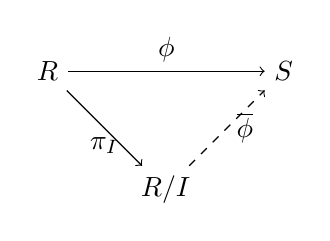
\begin{tikzpicture}
		\node (M) at (0,0) {$R$};
		\node (MS) at (3,0) {$S$};
		\node (Q) at (1.5,-1.5) {$R/I$};
		\draw[->, above] (M) to node {$\phi$} (MS);
		\draw[->, below] (M)  to node {$\pi_I$} (Q);
		\draw[->, right, dashed] (Q)  to node {$\overline{\phi}$} (MS);
		\end{tikzpicture}
	\end{center}
	Insbesondere gilt: Ist $\phi$ surjektiv, so induziert $\phi$ ein Isomorphismus
	\begin{align}
		R / \ker \phi \cong S. \notag
	\end{align}
\end{proposition}

\begin{proof}
	Siehe LAAG VIII.5.9.
\end{proof}

\begin{lemma}
	\proplbl{2_2_9}
	\begin{enumerate}
		\item Für $J \unlhd S$ ist $\phi^{-1}(J) \unlhd R$.
		\item Ist $\phi$ surjektiv, so liefert $J \mapsto \phi^{-1}(J)$ eine Bijektion $\Phi$ zwischen
		\begin{enumerate}
			\item Idealen von $S$, und
			\item Idealen von $R$, die $\ker \phi$ enthalten
		\end{enumerate}
	\end{enumerate}
\end{lemma}

\begin{proof}
	(vgl. LAAG VIII.5.5)
	Skizze:
	\begin{enumerate}
		\item $a \in \phi^{-1}(J)$, $r \in R$ $\Rightarrow \phi(ra) = \underbrace{\phi(r)}_{\in R}\underbrace{\phi(a)}_{\in J}\in J$
		\item Umkehrabbildung: $I \mapsto \phi(I)$
		\begin{itemize}
			\item $\phi(\phi^{-1}(J))=J\colon \phi$ surjektiv
			\item $\phi^{-1}(\phi(I)) = I\colon$ \propref{1_3_7}
			\item $I \unlhd R \Rightarrow \phi(I) \unlhd S: A \in I, s \in S \xRightarrow{\phi \text{ surjektiv}} s = \phi(r)$ mit $r \in R$:\\
			$\Rightarrow s \phi(a) = \phi(r)\phi(a) = \phi(ra)$ mit $ra \in I \Rightarrow s\phi(a) \in \phi(I)$
		\end{itemize}
	\end{enumerate}
\end{proof}

\begin{definition}[prim und maximal Ideal]
	\begin{enumerate}
		\item $I$ ist \begriff{prim} $:\Leftrightarrow \dot{I} \neq R$ und für $a,b \in R$ gilt:
		\begin{align}
			ab \in I \Rightarrow a \in I \vee b \in I\notag
		\end{align}
		\item $I$ ist \begriff{maximal} $:\Leftrightarrow I \neq R$ und $J \unlhd R$ mit
		\begin{align}
			I \subseteq J \subsetneq R\text{, so ist } I = J.
		\end{align}
	\end{enumerate}
\end{definition}

\begin{proposition}
	\proplbl{2_2_11}
	Sei $I \not\unlhd R$ %TODO do we have now a working not-ed \unlhd?
	\begin{enumerate}
		\item $I$ ist prim $\Leftrightarrow R/I$ ist nullteilerfrei
		\item $I$ ist maximal $\Leftrightarrow R/I$ ist Körper
		\item $I$ ist maximal $\Rightarrow I$ prim
	\end{enumerate}
\end{proposition}

\begin{proof} 
	\begin{enumerate}
		\item Beachte: $\pi_I(a)=0 \Leftrightarrow a \in I$\\
		``$\Rightarrow$'': $a,b \in R$ $\pi_I(a)\cdot\pi_I(b) = 0$\\
		$\Rightarrow 0 = \pi_I(a)\pi_I(b) = \pi_I(ab)$\\
		$\Rightarrow ab \in I \xRightarrow{I \text{ prim}} a \in I \vee b \in I$\\
		$\Rightarrow \pi_I(a) = 0 \vee \pi_I(b) = 0$\\
		``$\Leftarrow$'': $I$ nicht prim $\Rightarrow$ existiert $a,b \in R$ mit $ab \in I$, $a \not\in I$, $b \not \in I$\\
		$\Rightarrow$ $0 = \pi_I(ab) = \underbrace{\pi_I(a)}_{\neq 0}\underbrace{\pi_I(n)}_{\neq 0}$\\
		$\Rightarrow$ $R/I$ ist nicht nullteilerfrei
		\item $I$ maximal $\overset{\propref{2_2_9}b)}{\Longleftrightarrow}$ $R/I$ hat nur die Ideale $(0) = \pi_I(1)$ und $(1) = \pi_I(R)$ $\overset{\proplbl{2_2_9}d)}{\Longleftrightarrow}$ $R/I$ ist Körper %TODO here is somewhere a mistake, please check!
		\item folgt aus 1) $+$ 2), denn Körper sind nullteilerfrei!
	\end{enumerate}
\end{proof}

\begin{example}[Gegenbeispiel, dass die Umkehrung von \propref{2_2_11}c) nicht gilt!]
	In $R = \whole$: Ideale sind genau die Hauptideale
	\begin{itemize}
		\item $(n) = n\whole, n \in \natur_0$
		\item $(n)$ ist prim $\Rightarrow n$ Primzahl oder $n = 0$
		\item $(n)$ ist maximal $\Rightarrow n$ Primzahl
	\end{itemize}
\end{example}

\begin{proposition}
	Jedes echte Ideal $I \unlhd R$ ist in einem maximalen Ideal von $R$ enthalten.
\end{proposition}

\begin{proof}
	Lemma von Zorn. Die Vereinigung einer Kette echter Ideale ist wegen \propref{2_2_3}c)
	wieder ein echtes Ideal.
\end{proof}